% !TEX encoding = UTF-8 Unicode

\documentclass[a4paper]{article}

\usepackage{color}
\usepackage{url}
\usepackage[T2A]{fontenc} % enable Cyrillic fonts
\usepackage[utf8]{inputenc} % make weird characters work
\usepackage{graphicx}

\usepackage[english,serbian]{babel}
%\usepackage[english,serbianc]{babel} %ukljuciti babel sa ovim opcijama, umesto gornjim, ukoliko se koristi cirilica

\usepackage[unicode]{hyperref}
\hypersetup{colorlinks,citecolor=green,filecolor=green,linkcolor=blue,urlcolor=blue}

%\newtheorem{primer}{Пример}[section] %ćirilični primer
\newtheorem{primer}{Primer}[section]

\begin{document}

\title{Kvantna kriptografija\\ \small{Seminarski rad u okviru kursa\\Tehničko i naučno pisanje\\ Matematički fakultet}}

\author{Igor Glišović\\mi22292@alas.matf.bg.ac.rs\\\\ Željko Zekavičić\\mi22130@alas.matf.bg.ac.rs\\\\ Nađa Lazarević\\mi22175@alas.matf.bg.ac.rs\\\\ Ana Mladenović\\mi22119@alas.matf.bg.ac.rs\\\\}
\date{24.~oktobar 2017.}
\maketitle

\abstract{
U ovom tekstu je ukratko prikazana osnovna forma seminarskog rada. Obratite pažnju da je pored ove .pdf datoteke, u prilogu i odgovarajuća .tex datoteka, kao i .bib datoteka korišćena za generisanje literature. Na prvoj strani seminarskog rada su naslov, apstrakt i sadržaj, i to sve mora da stane na prvu stranu! Kako bi Vaš seminarski zadovoljio standarde i očekivanja, koristite uputstva i materijale sa predavanja na temu pisanja seminarskih radova. Ovo je samo šablon koji se odnosi na fizički izgled seminarskog rada (šablon koji \emph{morate} da ispoštujete!) kao i par tehničkih pomoćnih uputstava. 
\newpage

\tableofcontents

\newpage

\section{Uvod}

\section{Principi kvantne kriptografije}
Kvantna mehanika se zasniva na sledećim aspektima:
\begin{itemize}
\item aspekt prirodne neodređenosti, isprepletanosti - superpozicije, odnosno da se čestice koje postoje ne nalaze samo na jednom mestu (mogu se naći na dva mesta istovremeno)
\item aspekt kvantnog sprezanja, što znači da su dve nezavisne čestice uvek nerazdvojno povezane, čak iako ne postoji mogućnost njihovog međusobnog delovanja
\item delovanje jedne čestice na drugu, pa čak i odmeravanje, promeniće prirodu druge čestice
\end{itemize}
Ovi aspekti su ključni za kvantnu kriptografiju, jer obezbeđuju sigurnost očuvanja ključa.
\subsection{Kvantni računari}
Ključna razlika između klasičnih računara i kvantnih računara je vid predstavljanja podataka. Na klasičnim račuanrima, podaci se predstavljaju pomoću bitova (0,1), dok se na kvantnim predstavljaju u kvantnim bitovima - kubitima. Kubit može biti neka mikro ili nano čestica (foton, elektron, atom) i radi uz pomoć nekog mikrokontrolera koji će joj zadati sledeće stanje (smer rotacije). Sve informacije se kodiraju u tzv. kvantna stanja. U našem slučaju podatke prenosimo putem optičkih kablova, a osnovne čestice su fotoni. Fotoni se pri kretanju rotiraju pod nekim uglom, a kada se više fotona rotira u istom smeru, onda su oni polarizovani fotoni. Polarizacioni filteri propištaju isključivo fotone koji su polarizovani u jednom određenom smeru, a ostale blokiraju. Prepoznavanje promene smera je zapravo indikacija da neko pokušava da sazna informacije, jer je pokušao da sazna ključ, a samim tim promenio smer rotacije nekih kubita.


Potencijal kvantnih računara je veliki jer bi se za n-operacija kod klasičnog računara, sa istim brojem kubita kod kvantnog računara moglo uraditi $ 2^{n} $ operacija (eksponencijalno rastući kapacitet). 
\subsection{Kvantni protokoli}
Kvantni protokoli postoji zato što postoji razlika u distribuciji kvantnih ključeva, te razlikujemo nekoliko različitih protokola:
\begin{itemize}
\item BB84 protokol - prvi i najrasprostranjeniji protokol. Koristi jedan jednosmerni kvantni kanal i jedan dvosmerni javni kanal; bazira se na 4 neortogonalna stanja. 
\item B92 protokol - koristi 2 neortogonalna stanja.
\item E91 protokol - koristi isprepletani par fotona.
\item SARG04 - otporniji BB84.
\item Protokol šest stanja  - tri para ortogonalnih polarizacionih stanja (najnoviji, ali najmanje efikasan).
\end{itemize}
\begin{figure}[h]
\centering
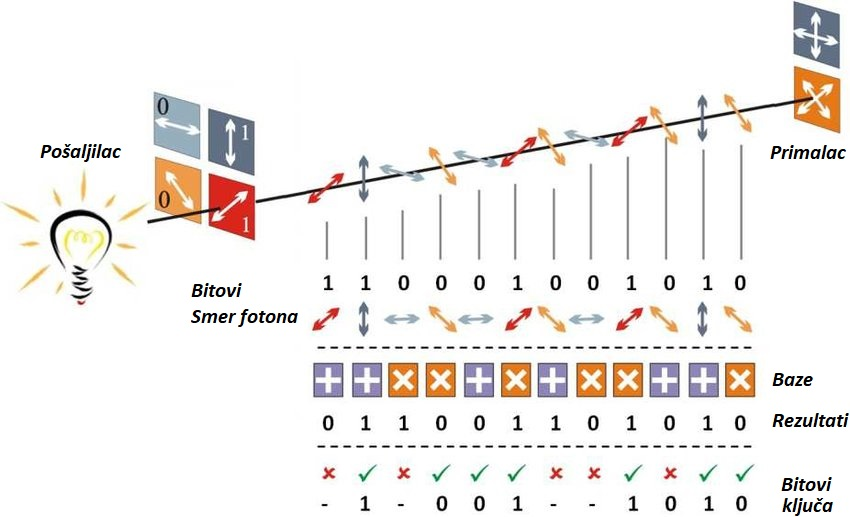
\includegraphics[width=0.8\textwidth]{bb84.jpg}
\caption{Metodika rada BB84 protokola}
\label{slike:prva}
\end{figure}\newpage 
\subsection{Kvantna razmena ključa}
Sigurni prenos informacija nemoguće je izvesti bez sigurnog prenosa ključa, stoga postoji nekoliko setova pravila koje koristimo pri razmeni ključeva, a mi ćemo navesti dva najosnovnija.
\begin{itemize}
 \item "Pripremi i izmeri" tip protokola                                                                                                                      - Zasniva se na aspektu neodređenosti kvantnih čestica i njihovog svojstva da promene stanje u odnosu na drugu česticu
 \item Protokoli zasnovani na isprepletanosti                                                                                                                        - Kombinovanje više kubita kako bismo otklonili mogućnost zamene greške prenosa (šumova) sa neovlašćenim napadom. 
\end{itemize}
 

\subsection{Vrste napada na sisteme i odbrana}
Postoji nekoliko vrsta napada na kvantne kriptografske sisteme, i to:
\begin{itemize}
\item "Middleman" (središnja osoba) napad - dešava se jer nismo obezbedili autentifikaciju u sistemu
\item PNS napad - koriste oslabljene laserske pulseve kako bi došli do male količine informacije
\item Hakerski napadi - ciljaju nesavršenost u implementacijama
protokola umesto samih protokola (najčešće koriste lažna stanja ili "Trojance")
\item DOS (Denial of Service) napad - blokiranje protoka informacije, "presretanje"
\end{itemize}
Kvantni kriptografski sistem biće siguran ako i samo ako obezbedimo da će svi delovi sistema raditi besprekorno. Moramo da se postaramo da nijedno treće lice ne može da pristupi uređajima za enkripciju/dekripciju koji se nalaze kod pošaljioca/primaoca informacije koje prenosimo. Pored toga moramo obezbediti da se svaki put generiše potpuno nasumična vrednost ključa (bez ikakve mogućnosti nalaska pravilnosti).  Na kraju, moramo obezbediti da naš komunikacioni medijum ima siguran proces autentifikacije (potvrda identiteta).


\section{Istorijat}	
\label{sec:termini_i_citiranje}


\section{Kvantna kriptografija danas}

\section{Zaključak}
\label{sec:zakljucak}


\newpage
\addcontentsline{toc}{section}{Literatura}
\appendix

\iffalse
\bibliography{seminarski} 
\bibliographystyle{plain}
\fi

\begin{thebibliography}{9}

\bibitem{laski2009software} J. Laski and W. Stanley. \emph{Software Verification and Analysis}. Springer- Verlag, London, 2009.

\bibitem{gcc} Free Software Foundation. GNU gcc, 2013. on-line at: http://gcc. gnu.org/.

\bibitem{haltingproblem} A. M. Turing. \emph{On Computable Numbers, with an application to the Entscheidungsproblem}. Proceedings of the London Mathematical Society, 2(42):230–265, 1936.


\end{thebibliography}


\appendix

\section{Dodatak}
Ovde pišem dodatne stvari, ukoliko za time ima potrebe.
Ovde pišem dodatne stvari, ukoliko za time ima potrebe.
Ovde pišem dodatne stvari, ukoliko za time ima potrebe.
Ovde pišem dodatne stvari, ukoliko za time ima potrebe.
Ovde pišem dodatne stvari, ukoliko za time ima potrebe.


\end{document}
